% This example is meant to be compiled with lualatex or xelatex
% The theme itself also supports pdflatex
\PassOptionsToPackage{unicode}{hyperref}
\documentclass[aspectratio=1610, 12pt]{beamer}

% Warning, if another latex run is needed
% \usepackage[aux]{rerunfilecheck}

% just list chapters and sections in the toc, not subsections or smaller
\setcounter{tocdepth}{1}

%------------------------------------------------------------------------------
%------------------------------ Fonts, Unicode, Language ----------------------
%------------------------------------------------------------------------------
\usepackage{fontspec}
\defaultfontfeatures{Ligatures=TeX}  % -- becomes en-dash etc.

% german language
\usepackage{polyglossia}
\setdefaultlanguage{german}

% for english abstract and english titles in the toc
\setotherlanguages{english}

% intelligent quotation marks, language and nesting sensitive
\usepackage[autostyle]{csquotes}

% microtypographical features, makes the text look nicer on the small scale
\usepackage{microtype}

%------------------------------------------------------------------------------
%------------------------ Math Packages and settings --------------------------
%------------------------------------------------------------------------------

\usepackage{amsmath}
\usepackage{amssymb}
\usepackage{mathtools}
\usepackage{bbold}

% Enable Unicode-Math and follow the ISO-Standards for typesetting math
\usepackage[
  math-style=ISO,
  bold-style=ISO,
  sans-style=italic,
  nabla=upright,
  partial=upright,
]{unicode-math}
\setmathfont{Latin Modern Math}

% nice, small fracs for the text with \sfrac{}{}
\usepackage{xfrac}


%------------------------------------------------------------------------------
%---------------------------- Numbers and Units -------------------------------
%------------------------------------------------------------------------------

\usepackage[
  locale=DE,
  separate-uncertainty=true,
  per-mode=symbol-or-fraction,
]{siunitx}
\sisetup{math-micro=\text{µ},text-micro=µ}
% \sisetup{tophrase={{ to }}}
%------------------------------------------------------------------------------
%-------------------------------- tables  -------------------------------------
%------------------------------------------------------------------------------

\usepackage{booktabs}       % \toprule, \midrule, \bottomrule, etc

%------------------------------------------------------------------------------
%-------------------------------- graphics -------------------------------------
%------------------------------------------------------------------------------

\usepackage{graphicx}
%\usepackage{rotating}
\usepackage{grffile}
\usepackage{tikz}
\usepackage{circuitikz}
\usepackage{tikz-feynman}
\usepackage{subcaption}

% allow figures to be placed in the running text by default:
\usepackage{scrhack}
\usepackage{float}
\floatplacement{figure}{htbp}
\floatplacement{table}{htbp}

% keep figures and tables in the section
\usepackage[section, below]{placeins}

% smileys
\usepackage{MnSymbol,wasysym}

%------------------------------------------------------------------------------
%---------------------- customize list environments ---------------------------
%------------------------------------------------------------------------------

\usepackage{enumitem}
\usepackage{listings}
\usepackage{hepunits}

\usepackage{pdfpages}
%------------------------------------------------------------------------------
%------------------------------ Bibliographie ---------------------------------
%------------------------------------------------------------------------------

\usepackage[
  backend=biber,   % use modern biber backend
  autolang=hyphen, % load hyphenation rules for if language of bibentry is not
                   % german, has to be loaded with \setotherlanguages
                   % in the references.bib use langid={en} for english sources
]{biblatex}
\addbibresource{references.bib}  % the bib file to use
\DefineBibliographyStrings{german}{andothers = {{et\,al\adddot}}}  % replace u.a. with et al.


% Load packages you need here
% \usepackage{polyglossia}
% \setmainlanguage{german}

\usepackage{csquotes}


% \usepackage{amsmath}
% \usepackage{amssymb}
% \usepackage{mathtools}

\usepackage{hyperref}
\usepackage{bookmark}

% load the theme after all packages

\usetheme[
  showtotalframes, % show total number of frames in the footline
]{tudo}

% Put settings here, like
\unimathsetup{
  math-style=ISO,
  bold-style=ISO,
  nabla=upright,
  partial=upright,
  mathrm=sym,
}

% \setbeamertemplate{itemize item}{\scriptsize$\blacktriangleright$}
% \setbeamertemplate{itemize subitem}{\scriptsize$\blacktriangleright$}

%Titel:
\title{Understanding the alignment of LHCb's SciFi Tracker}
%Autor
\author[N.Breer]{Nils Breer*, Sophie Hollitt, Johannes Albrecht}
%Lehrstuhl/Fakultät
\institute{Technische Universität Dortmund, Fakultät Physik}
%Titelgrafik muss ich einfueren!!!
%\titlegraphic{\includegraphics[width=0.3\textwidth]{content/Bilder/interferenz.jpg}}
\date{08.03.2023}

\begin{document}
\maketitle

\begin{frame}\frametitle{Overview}
  \begin{itemize}
    \item $\bullet$\, The SciFi Detector Upgrade
    \item $\bullet$\, Alignment how to
    \item $\bullet$\, Analysis of SciFi quarters
  \end{itemize}
\end{frame}

\begin{frame}\frametitle{The Scintillating Fibre Tracker}
  \begin{columns}
    \begin{column}[c]{0.48\textwidth}
      \begin{figure}
        \subfloat[]{%
          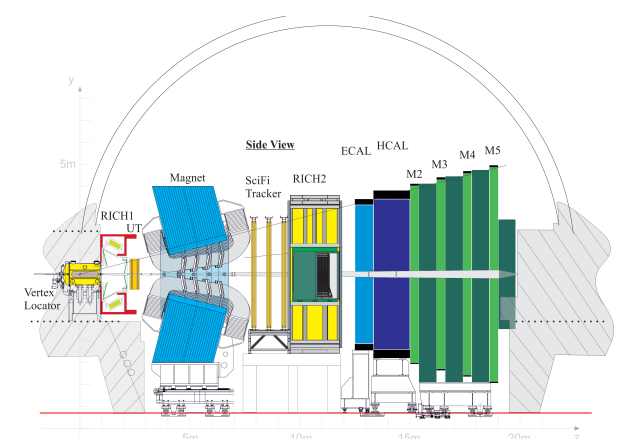
\includegraphics[clip,width=0.65\columnwidth]{logos/LHCb.png}%
        }

        \subfloat[]{%
          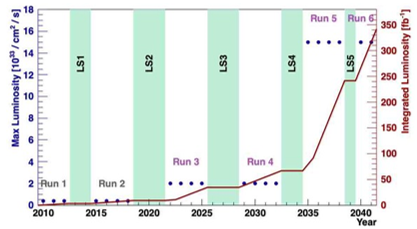
\includegraphics[clip,width=0.65\columnwidth]{logos/lumi_lhcb.png}%
        }

      \end{figure}
    \end{column}
    \begin{column}[c]{0.48\textwidth}
      \begin{itemize}
        \item $\bullet$\, Higher luminosity
        \begin{itemize}
          \item $\bullet$\, detector must operate well with expected radiation damage
        \end{itemize}
        \item $\bullet$\, detector readout electronics need to operate at 40 MHz, 25ns usable time per collision
        \item $\bullet$\, tracking efficiency and hit detection improvements aim for about 98\% hit detection rate
      \end{itemize}
    \end{column}
  \end{columns}
\end{frame}

\begin{frame}\frametitle{The Scintillating Fibre Tracker}
  \begin{columns}
    \begin{column}[c]{0.48\textwidth}
      \begin{figure}
        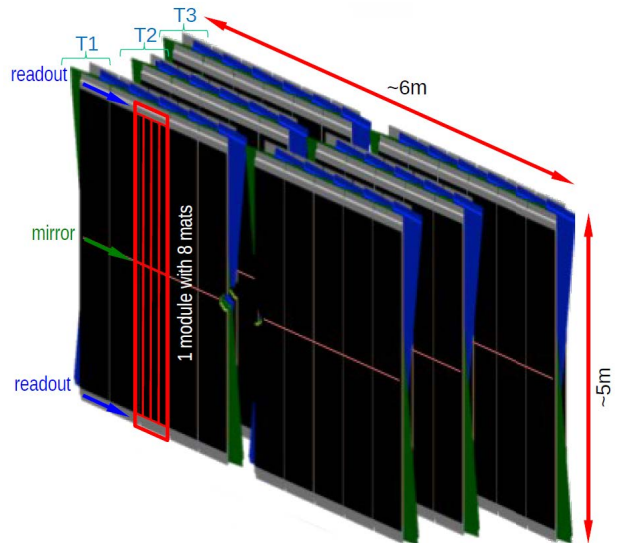
\includegraphics[width=0.9\textwidth]{logos/scifi.png}
        \caption{Visualization of the SciFi tracking stations.}
      \end{figure}
    \end{column}
    \begin{column}{0.48\textwidth}
      \begin{itemize}
        \item $\bullet$\, single detector type vs. IT + OT
        \item $\bullet$\, less timing information needed for readout
        \item $\bullet$\, less detector material
        \begin{itemize}
          \item $\bullet$\, less multiple scattering and material interactions
        \end{itemize}
        \item $\bullet$\, SiPM technology improvements yield better resolution and speed
      \end{itemize}
    \end{column}
  \end{columns}
\end{frame}

\begin{frame}\frametitle{What is Alignment?}
  \begin{columns}
    \begin{column}[c]{0.48\textwidth}
      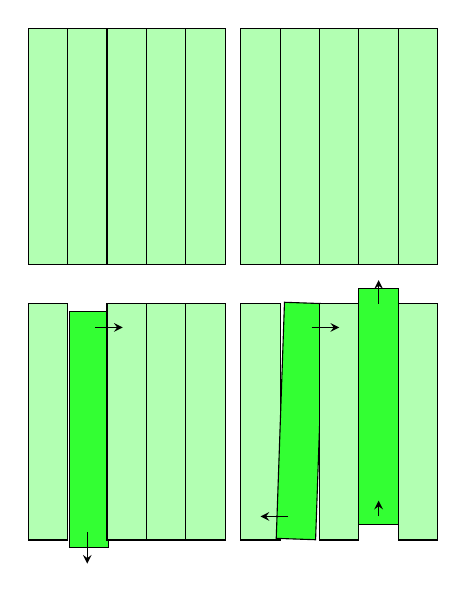
\begin{tikzpicture}
  % this is the ideal detector
  \node[rectangle,
      draw = black,
      % text = ,
      fill = green!30!white,
      minimum width = 0.5cm,
      minimum height = 3cm] (r) at (0,0) {};
  \node[rectangle,
      draw = black,
      % text = ,
      fill = green!80!white,
      minimum width = 0.5cm,
      minimum height = 3cm] (r) at (0.525,-0.1) {};
  \node[rectangle,
      draw = black,
      % text = ,
      fill = green!30!white,
      minimum width = 0.5cm,
      minimum height = 3cm] (r) at (1,0) {};
  \node[rectangle,
      draw = black,
      % text = ,
      fill = green!30!white,
      minimum width = 0.5cm,
      minimum height = 3cm] (r) at (1.5,0) {};
  \node[rectangle,
      draw = black,
      % text = ,
      fill = green!30!white,
      minimum width = 0.5cm,
      minimum height = 3cm] (r) at (2,0) {};

  \node[rectangle,
      draw = black,
      % text = ,
      fill = green!30!white,
      minimum width = 0.5cm,
      minimum height = 3cm] (r) at (2.7,0) {};
  \node[rectangle,
      draw = black,
      % text = ,
      fill = green!80!white,
      rotate around = {-2:(3.2,0)},
      minimum width = 0.5cm,
      minimum height = 3cm] (r) at (3.2,-0.1) {};
  % \draw (2.7,0) -- (5.7,0);
  \node[rectangle,
      draw = black,
      % text = ,
      fill = green!30!white,
      minimum width = 0.5cm,
      minimum height = 3cm] (r) at (3.7,0) {};
  \node[rectangle,
      draw = black,
      % text = ,
      fill = green!80!white,
      minimum width = 0.5cm,
      minimum height = 3cm] (r) at (4.2,0.2) {};
  \node[rectangle,
      draw = black,
      % text = ,
      fill = green!30!white,
      minimum width = 0.5cm,
      minimum height = 3cm] (r) at (4.7,0) {};

% now below it the physical detector
\node[rectangle,
    draw = black,
    % text = ,
    fill = green!30!white,
    minimum width = 0.5cm,
    minimum height = 3cm] (r) at (0,3.5) {};
\node[rectangle,
    draw = black,
    % text = ,
    fill = green!30!white,
    minimum width = 0.5cm,
    minimum height = 3cm] (r) at (0.5,3.5) {};
\node[rectangle,
    draw = black,
    % text = ,
    fill = green!30!white,
    minimum width = 0.5cm,
    minimum height = 3cm] (r) at (1,3.5) {};
\node[rectangle,
    draw = black,
    % text = ,
    fill = green!30!white,
    minimum width = 0.5cm,
    minimum height = 3cm] (r) at (1.5,3.5) {};
\node[rectangle,
    draw = black,
    % text = ,
    fill = green!30!white,
    minimum width = 0.5cm,
    minimum height = 3cm] (r) at (2,3.5) {};

\node[rectangle,
    draw = black,
    % text = ,
    fill = green!30!white,
    minimum width = 0.5cm,
    minimum height = 3cm] (r) at (2.7,3.5) {};
\node[rectangle,
    draw = black,
    % text = ,
    fill = green!30!white,
    minimum width = 0.5cm,
    minimum height = 3cm] (r) at (3.2,3.5) {};
\node[rectangle,
    draw = black,
    % text = ,
    fill = green!30!white,
    minimum width = 0.5cm,
    minimum height = 3cm] (r) at (3.7,3.5) {};
\node[rectangle,
    draw = black,
    % text = ,
    fill = green!30!white,
    minimum width = 0.5cm,
    minimum height = 3cm] (r) at (4.2,3.5) {};
\node[rectangle,
    draw = black,
    % text = ,
    fill = green!30!white,
    minimum width = 0.5cm,
    minimum height = 3cm] (r) at (4.7,3.5) {};

% draw arrows indicating the movement
% x and y translation
\draw [-stealth] (0.6,1.2) -- (0.95,1.2);
\draw [-stealth] (0.5,-1.4) -- (0.5,-1.8);

% rotation
\draw [-stealth] (3.35,1.2) -- (3.7,1.2);
\draw [-stealth] (3.05,-1.2) -- (2.7,-1.2);
% single translation
\draw [-stealth] (4.2,1.5) -- (4.2,1.8);
\draw [-stealth] (4.2,-1.2) -- (4.2,-1);

\end{tikzpicture}

    \end{column}
    \begin{column}[c]{0.48\textwidth}
      \begin{itemize}
        \item $\bullet$\, top: ideal detector, bottom: physical detector
        \item $\bullet$\, Surveys are used to find the rotation and position of each detector component
        \item $\bullet$\, Are used as starting positions for software alignment (this talk!)
      \end{itemize}
    \end{column}
  \end{columns}
\end{frame}

\begin{frame}\frametitle{Alignment: track fits with the Kalman Filter}
  \begin{columns}
    \begin{column}[c]{0.48\textwidth}
      \begin{figure}
        \centering
        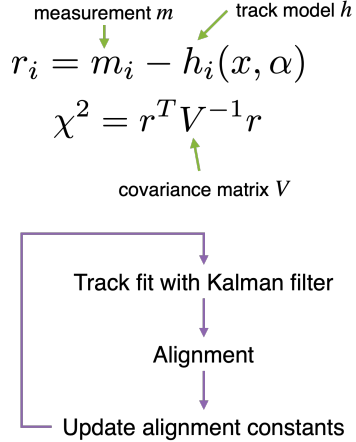
\includegraphics[width=\columnwidth]{logos/kalman.png}
        \caption{Alignment with Kalman Filter.}
      \end{figure}
    \end{column}
    \begin{column}[c]{0.48\textwidth}
      \begin{itemize}
        \item $\bullet$\, Minimise $\chi^2$ with respect to the track parameters for the track fit
        \item $\bullet$\, Minimise $\chi^2$ with respect to the alignment parameters $\alpha$ during the alignment
        \item $\bullet$\, Update the alignment constants $\alpha$ and repeat until convergence criterium for $\chi^2$ is reached
      \end{itemize}
    \end{column}
  \end{columns}
\end{frame}

\begin{frame}\frametitle{Alignment versions in use}
  \begin{columns}
    \begin{column}[c]{0.33\textwidth}
      \begin{itemize}
        \item V1:
        \begin{itemize}
          \item use full length Modules
          \item alignable degrees of freedom: Tx Rz (x translation, rotation around z \to beam pipe axis)
        \end{itemize}
      \end{itemize}
    \end{column}
    \begin{column}[c]{0.33\textwidth}
      \begin{itemize}
        \item $\text{low} \mu$:
        \begin{itemize}
          \item use half modules
          \item uses VELO alignment on run 256145 data
          \item $\mu =$ look it up
        \end{itemize}
      \end{itemize}
    \end{column}
    \begin{column}[c]{0.33\textwidth}
      \begin{itemize}
        \item V2:
        \begin{itemize}
          \item newest alignment version
          \item half modules (top half and bottom half)
          \item uses newest time alignment
          \item utilizes VELO alignment from run 256145
          \item $\mu \approx 2.26$ (value taken from run database)
        \end{itemize}
      \end{itemize}
    \end{column}
  \end{columns}
\end{frame}

\begin{frame}\frametitle{Why analyse the quarters separately?}
  \begin{itemize}
    \item $\bullet$\, perfomance in each quarter might be very different from one another
    \item $\bullet$\, \to $\chi^2$ per layer might be different from $\chi^2$ per quarter
    \item $\bullet$\, v2 alignment shows improvements from v1 alignment but not across the whole SciFi
    \item $\bullet$\, find and resolve possible issues is easier
  \end{itemize}
\end{frame}

\begin{frame}\frametitle{Summary of Metrics from alignments in Quarter 0}
  This hints that something is not right in Q0
  \begin{columns}
    \begin{column}[c]{0.48\textwidth}
      \begin{figure}
        \centering
        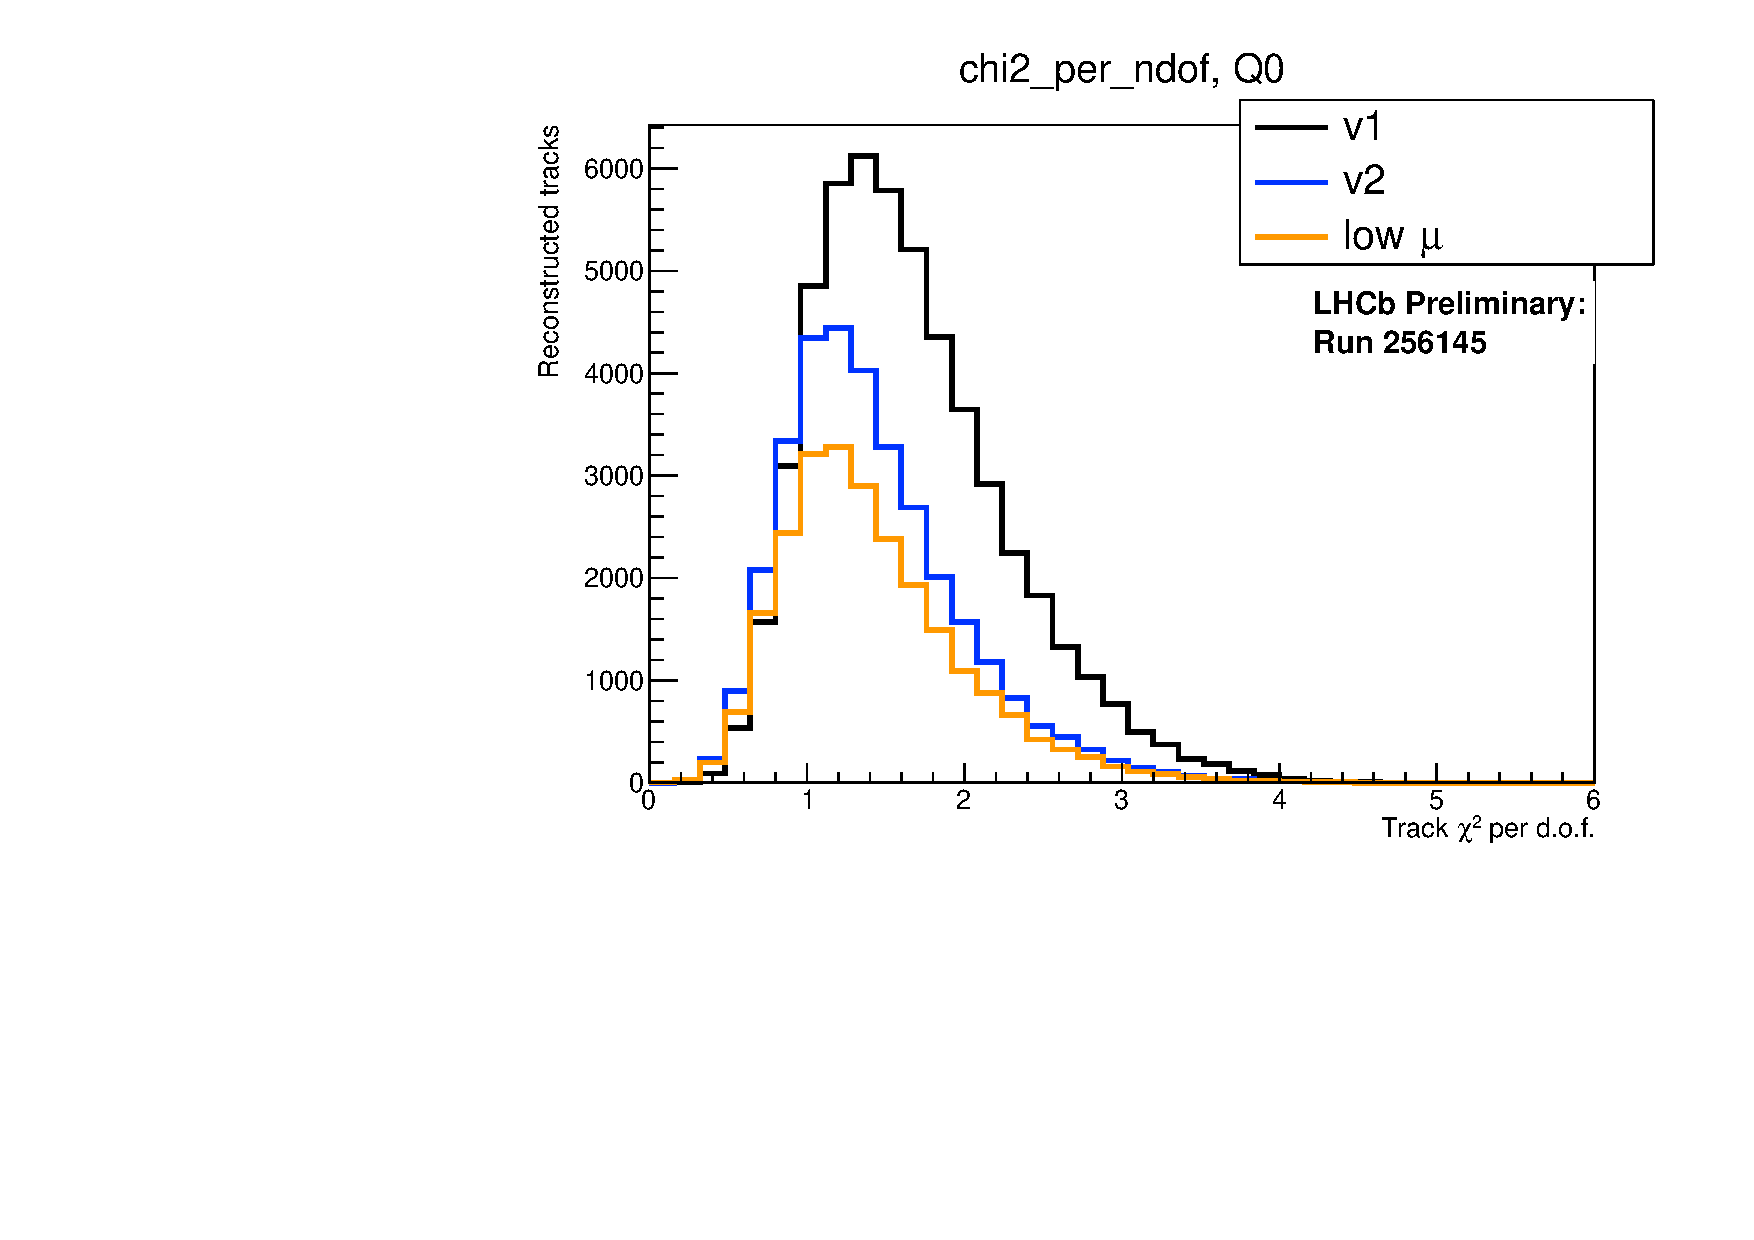
\includegraphics[width=0.9\textwidth]{2023-mar-9-DPG/chi2_per_ndof_Q0.pdf}
        \caption{track $\chi^2$ per dof comparing each alignment for Quarter 0.}
      \end{figure}
    \end{column}
    \begin{column}{0.48\textwidth}
      \begin{figure}
        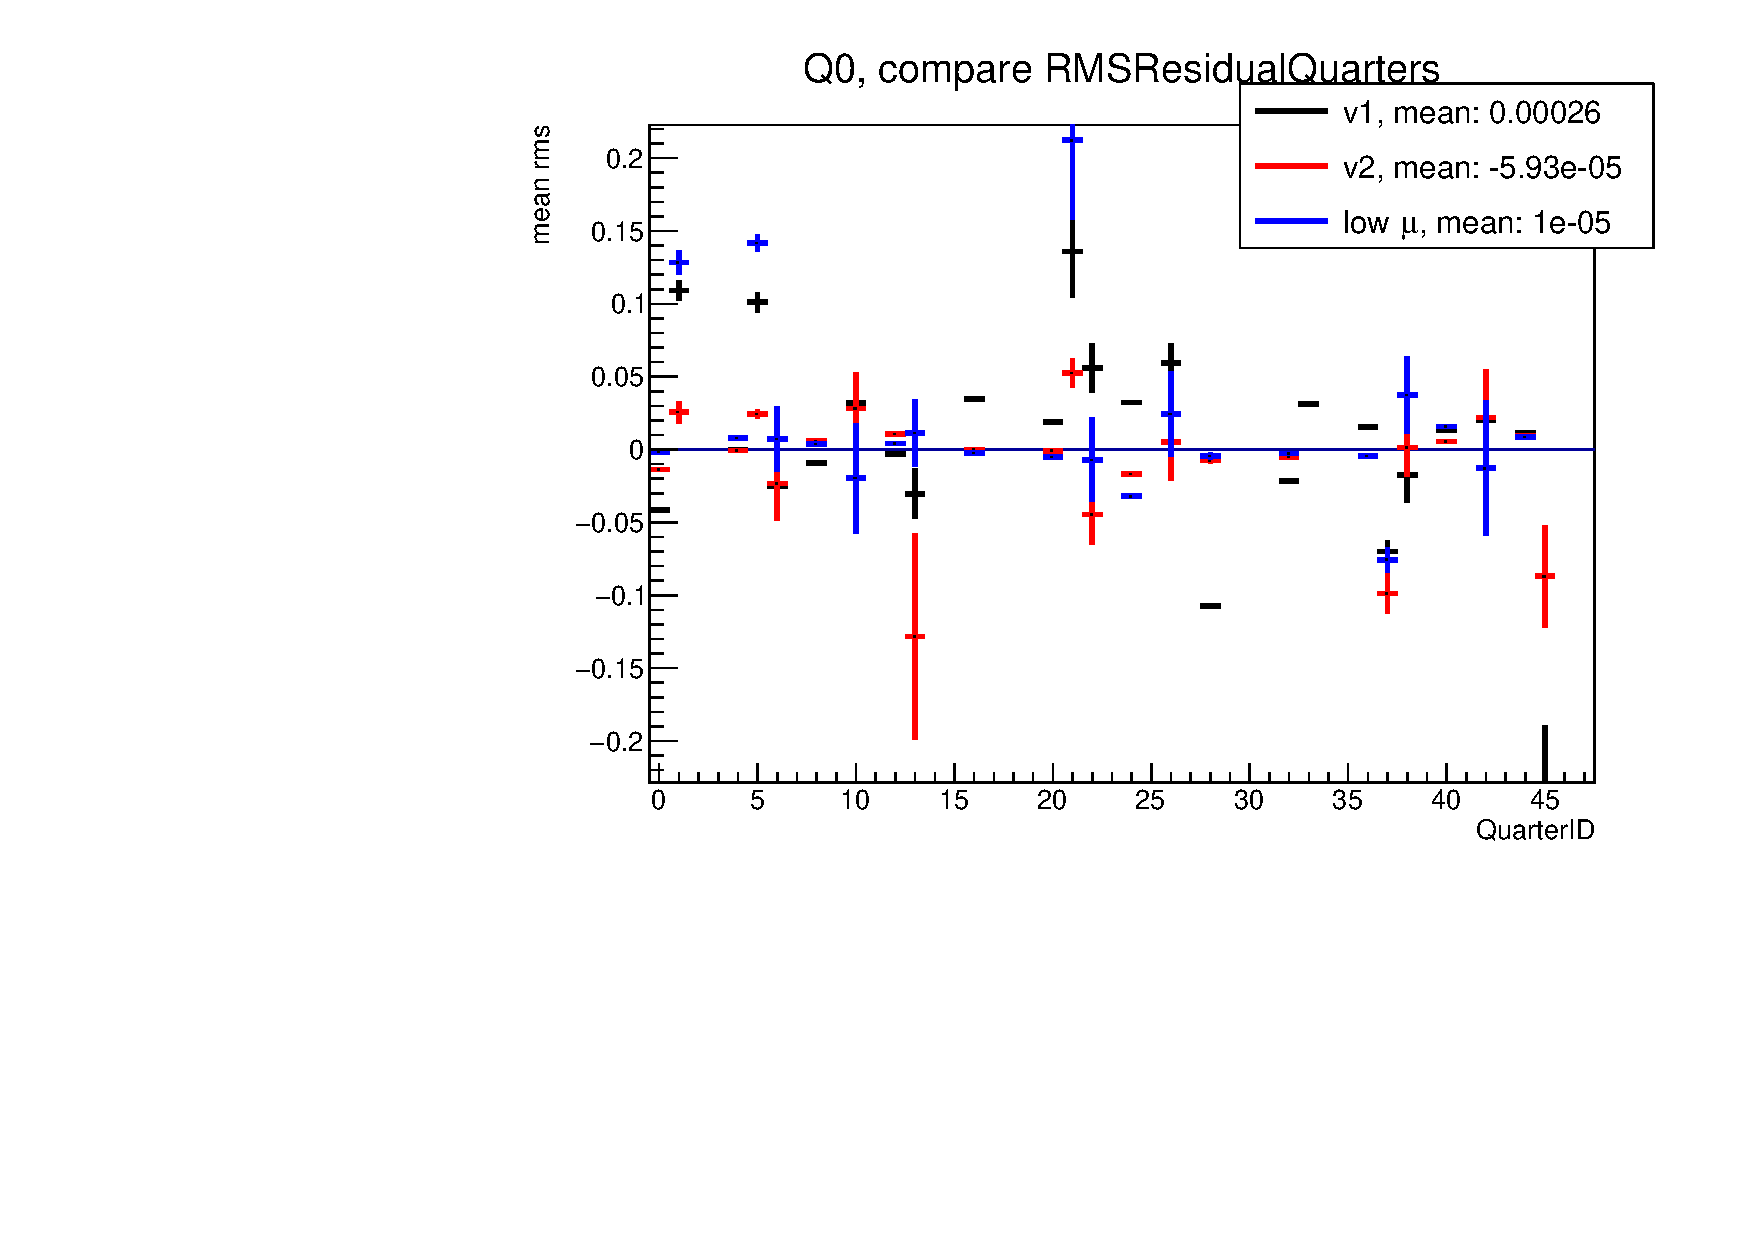
\includegraphics[width=0.9\textwidth]{2023-mar-9-DPG/RMSResidualQuarters_Q0.pdf}
        \caption{Residual in each module for each alignment in Quarter 0.}
      \end{figure}
    \end{column}
  \end{columns}
\end{frame}

\begin{frame}\frametitle{Summary of Metrics from alignments in Quarter 1}
  \begin{columns}
    \begin{column}[c]{0.48\textwidth}
      \begin{figure}
        \centering
        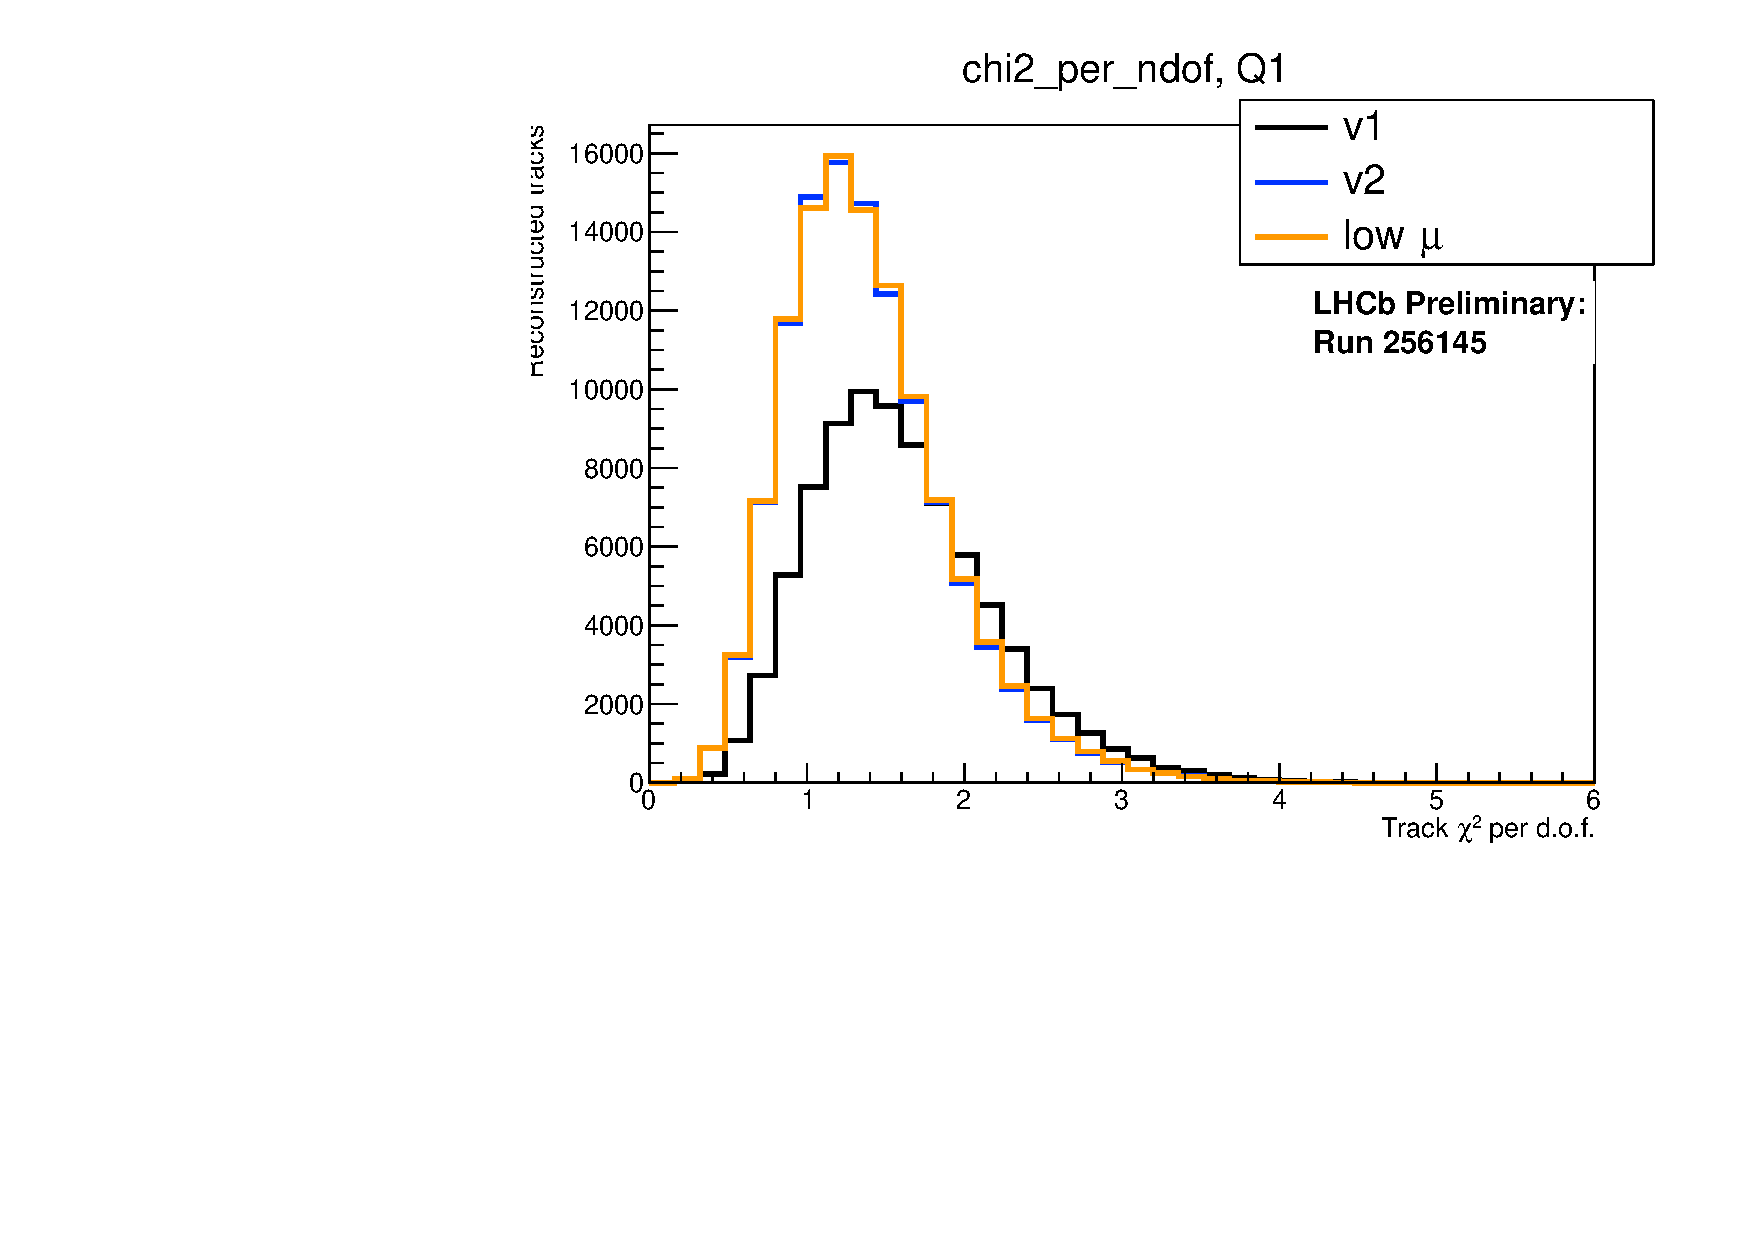
\includegraphics[width=0.9\textwidth]{2023-mar-9-DPG/chi2_per_ndof_Q1.pdf}
        \caption{track $\chi^2$ per dof comparing each alignment for Quarter 1.}
      \end{figure}
    \end{column}
    \begin{column}{0.48\textwidth}
      \begin{figure}
        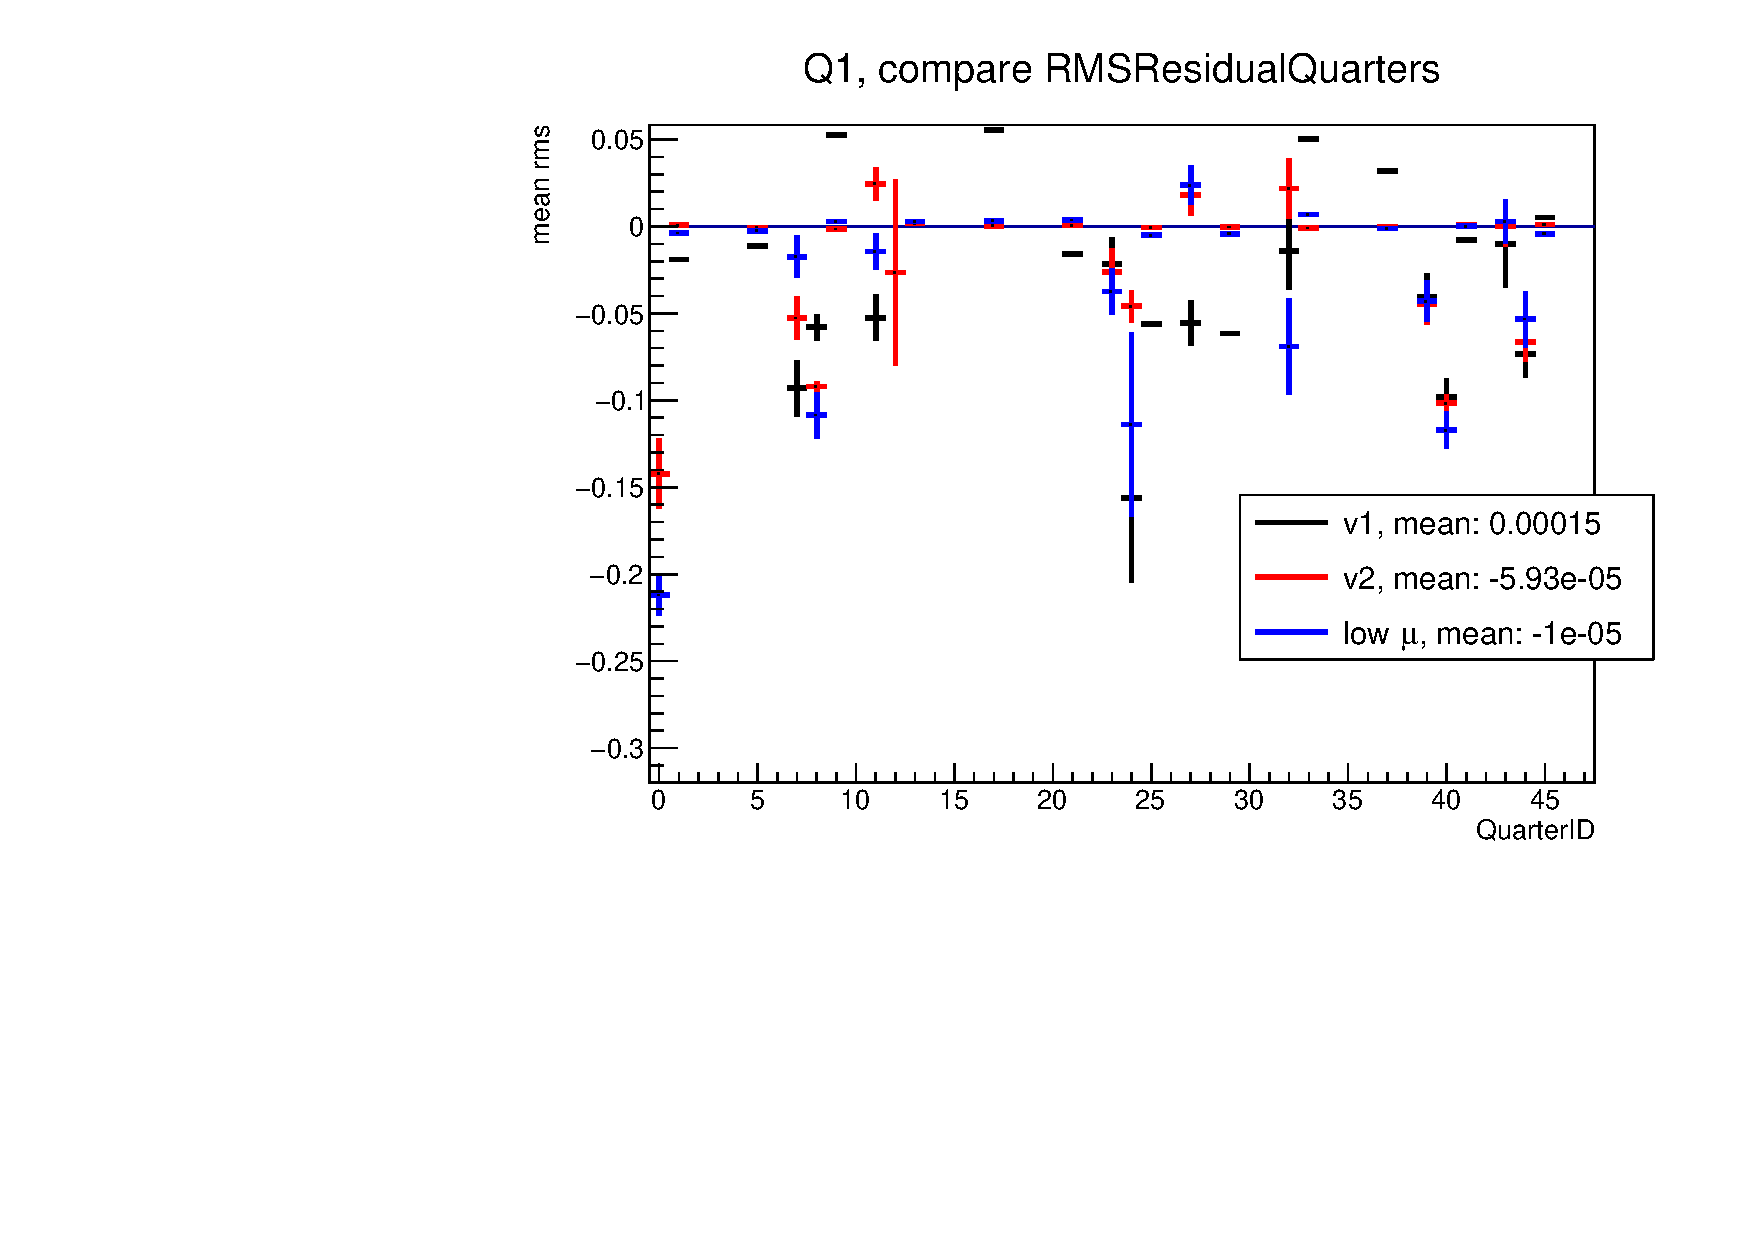
\includegraphics[width=0.9\textwidth]{2023-mar-9-DPG/RMSResidualQuarters_Q1.pdf}
        \caption{Residual in each module for each alignment in Quarter 1.}
      \end{figure}
    \end{column}
  \end{columns}
\end{frame}

\begin{frame}\frametitle{Summary of Metrics from alignments in Quarter 2}
  \begin{columns}
    \begin{column}[c]{0.48\textwidth}
      \begin{figure}
        \centering
        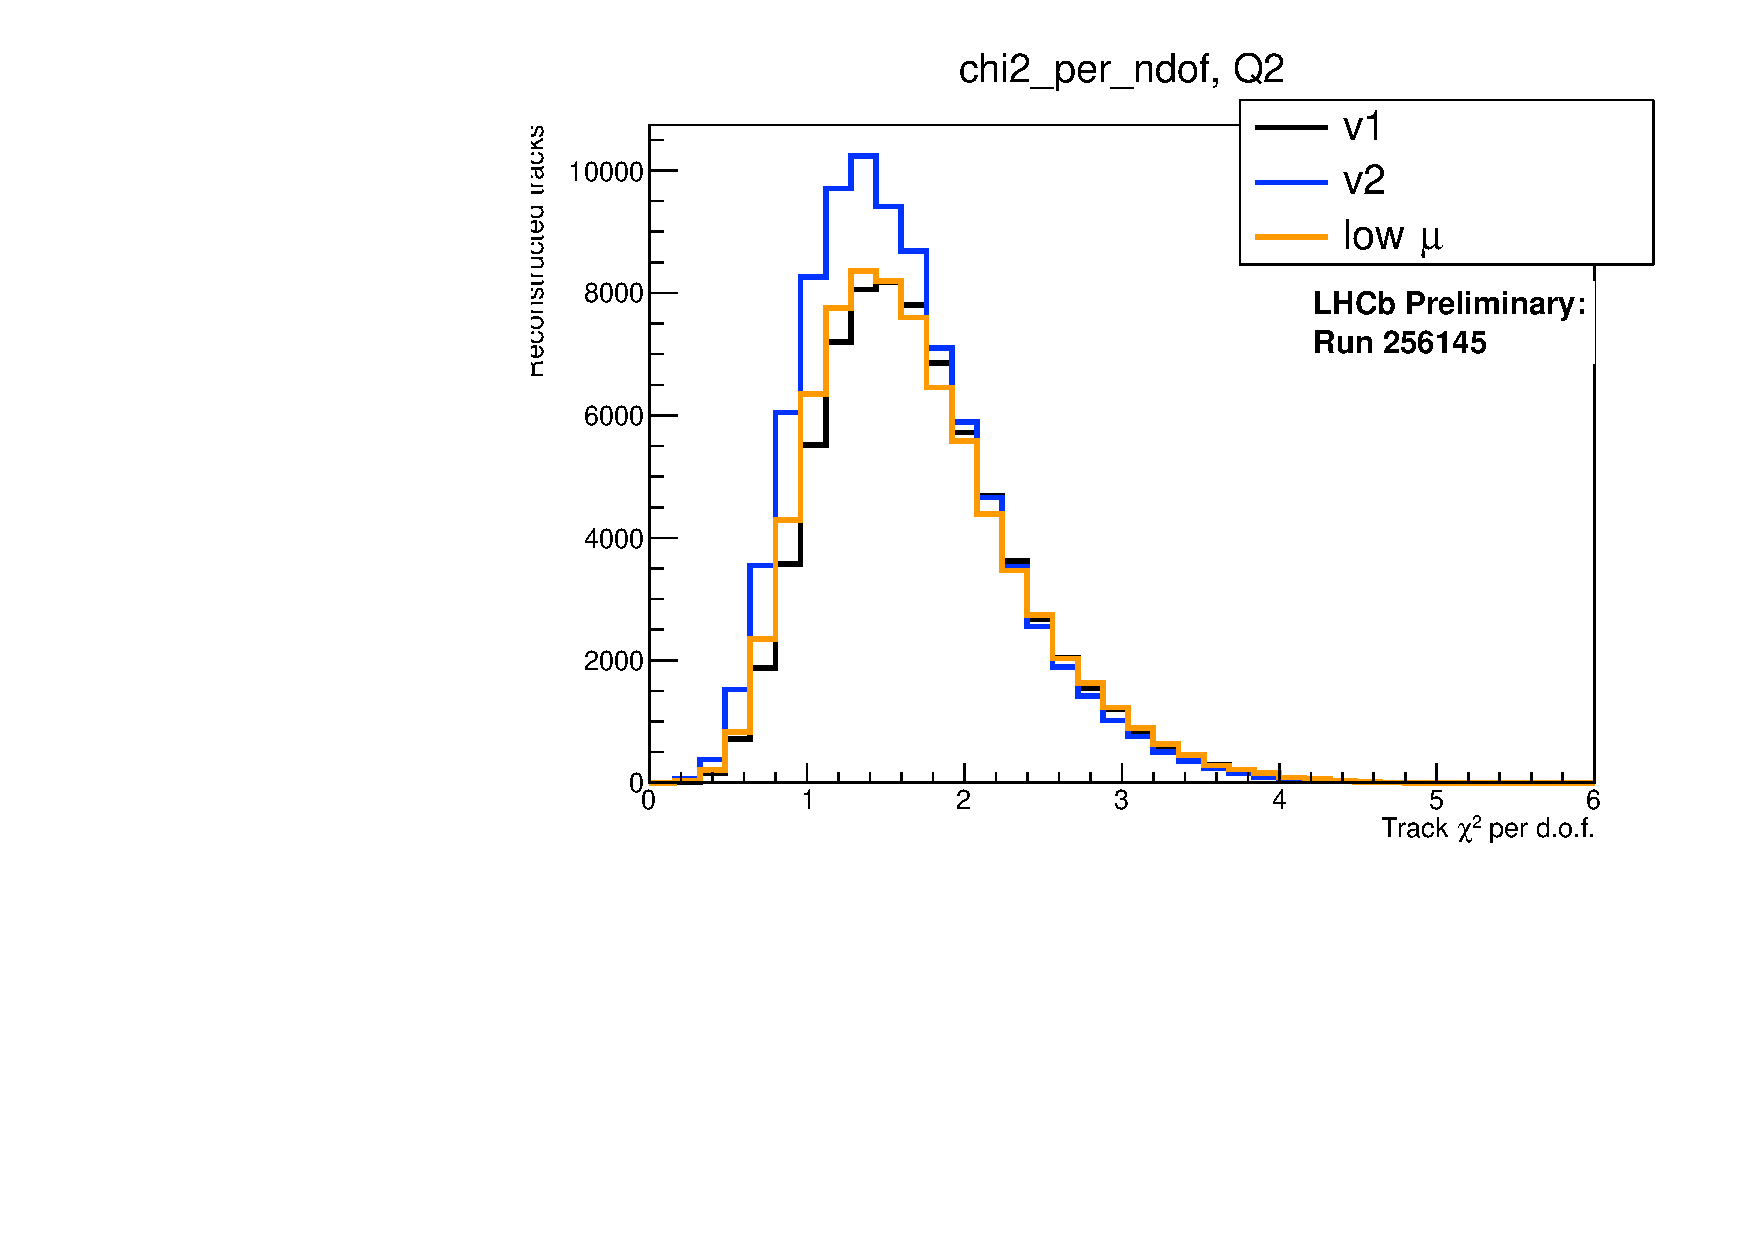
\includegraphics[width=0.9\textwidth]{2023-mar-9-DPG/chi2_per_ndof_Q2.pdf}
        \caption{track $\chi^2$ per dof comparing each alignment for Quarter 2.}
      \end{figure}
    \end{column}
    \begin{column}{0.48\textwidth}
      \begin{figure}
        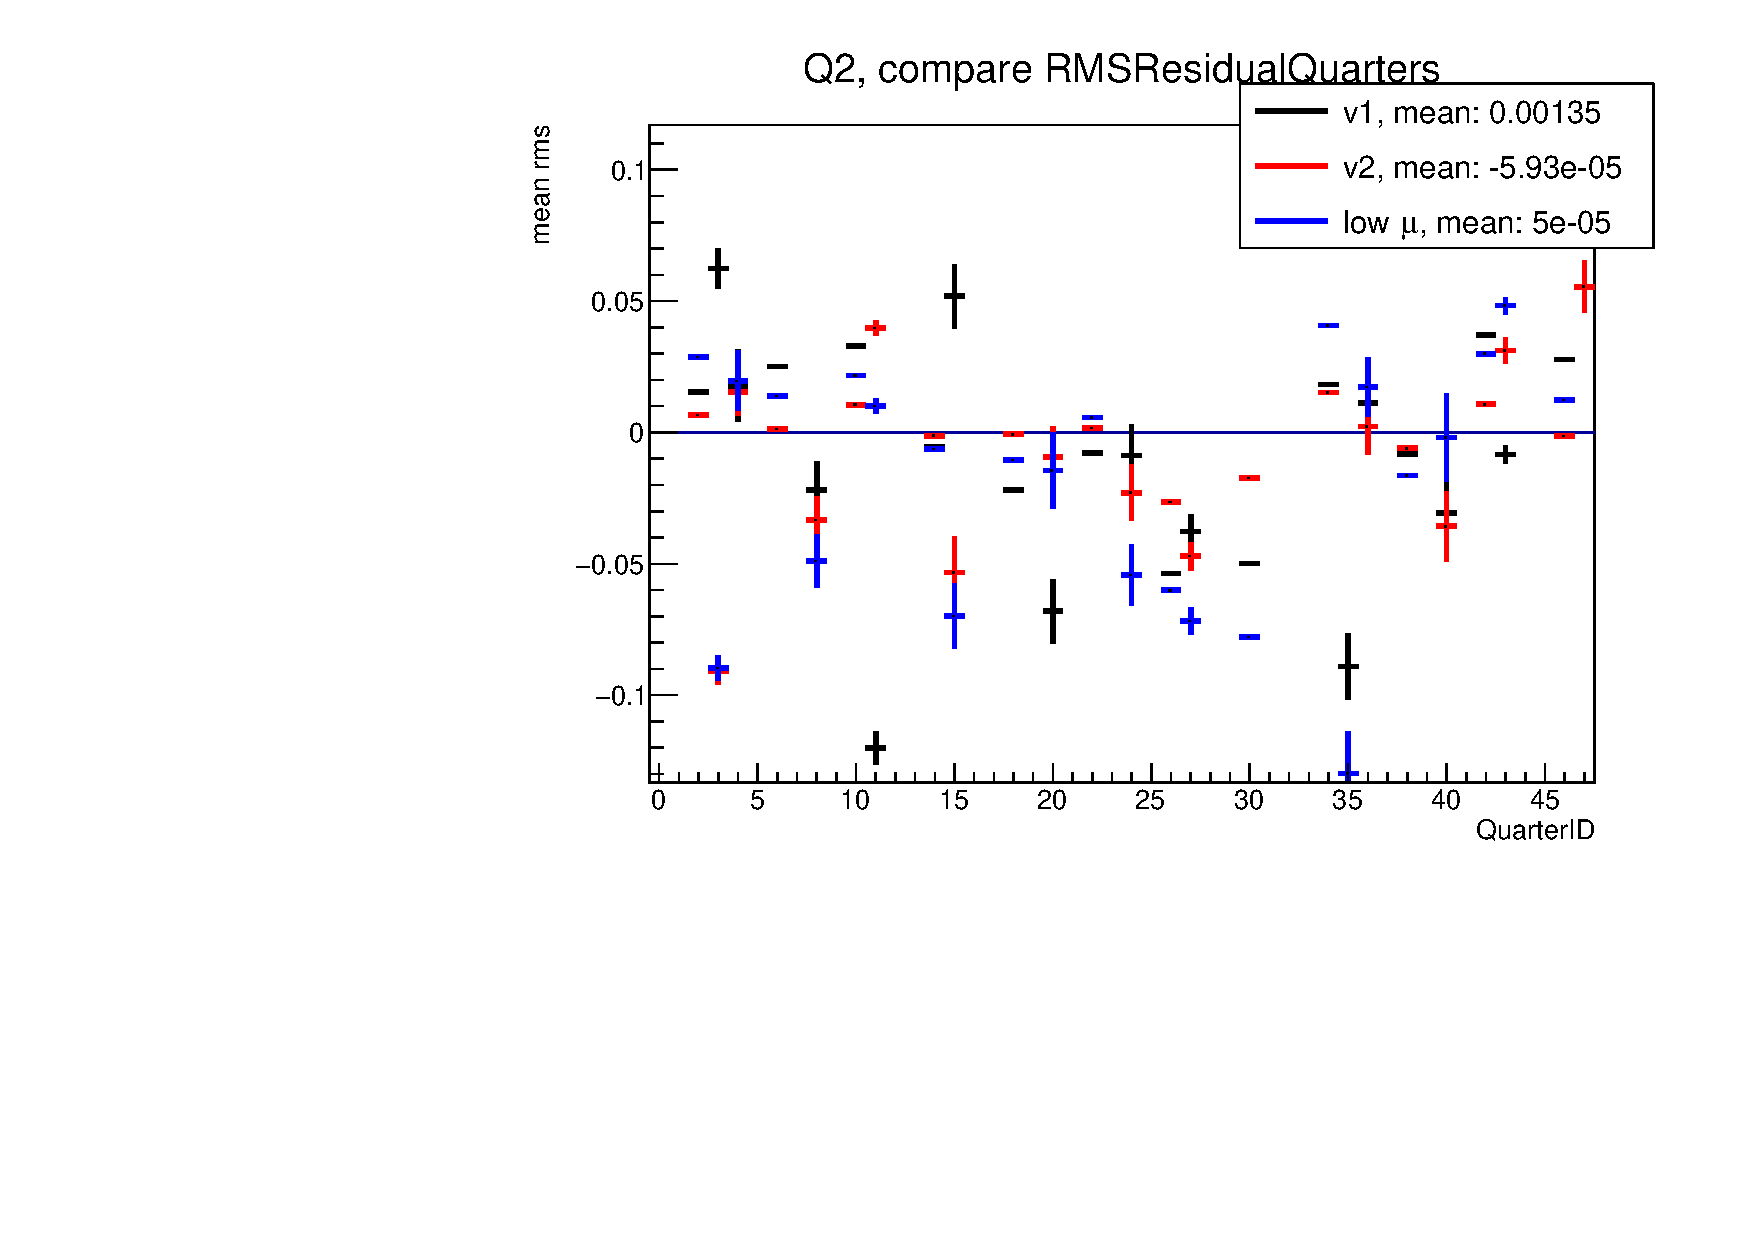
\includegraphics[width=0.9\textwidth]{2023-mar-9-DPG/RMSResidualQuarters_Q2.pdf}
        \caption{Residual in each module for each alignment in Quarter 2.}
      \end{figure}
    \end{column}
  \end{columns}
\end{frame}

\begin{frame}\frametitle{Summary of Metrics from alignments in Quarter 3}
  \begin{columns}
    \begin{column}[c]{0.48\textwidth}
      \begin{figure}
        \centering
        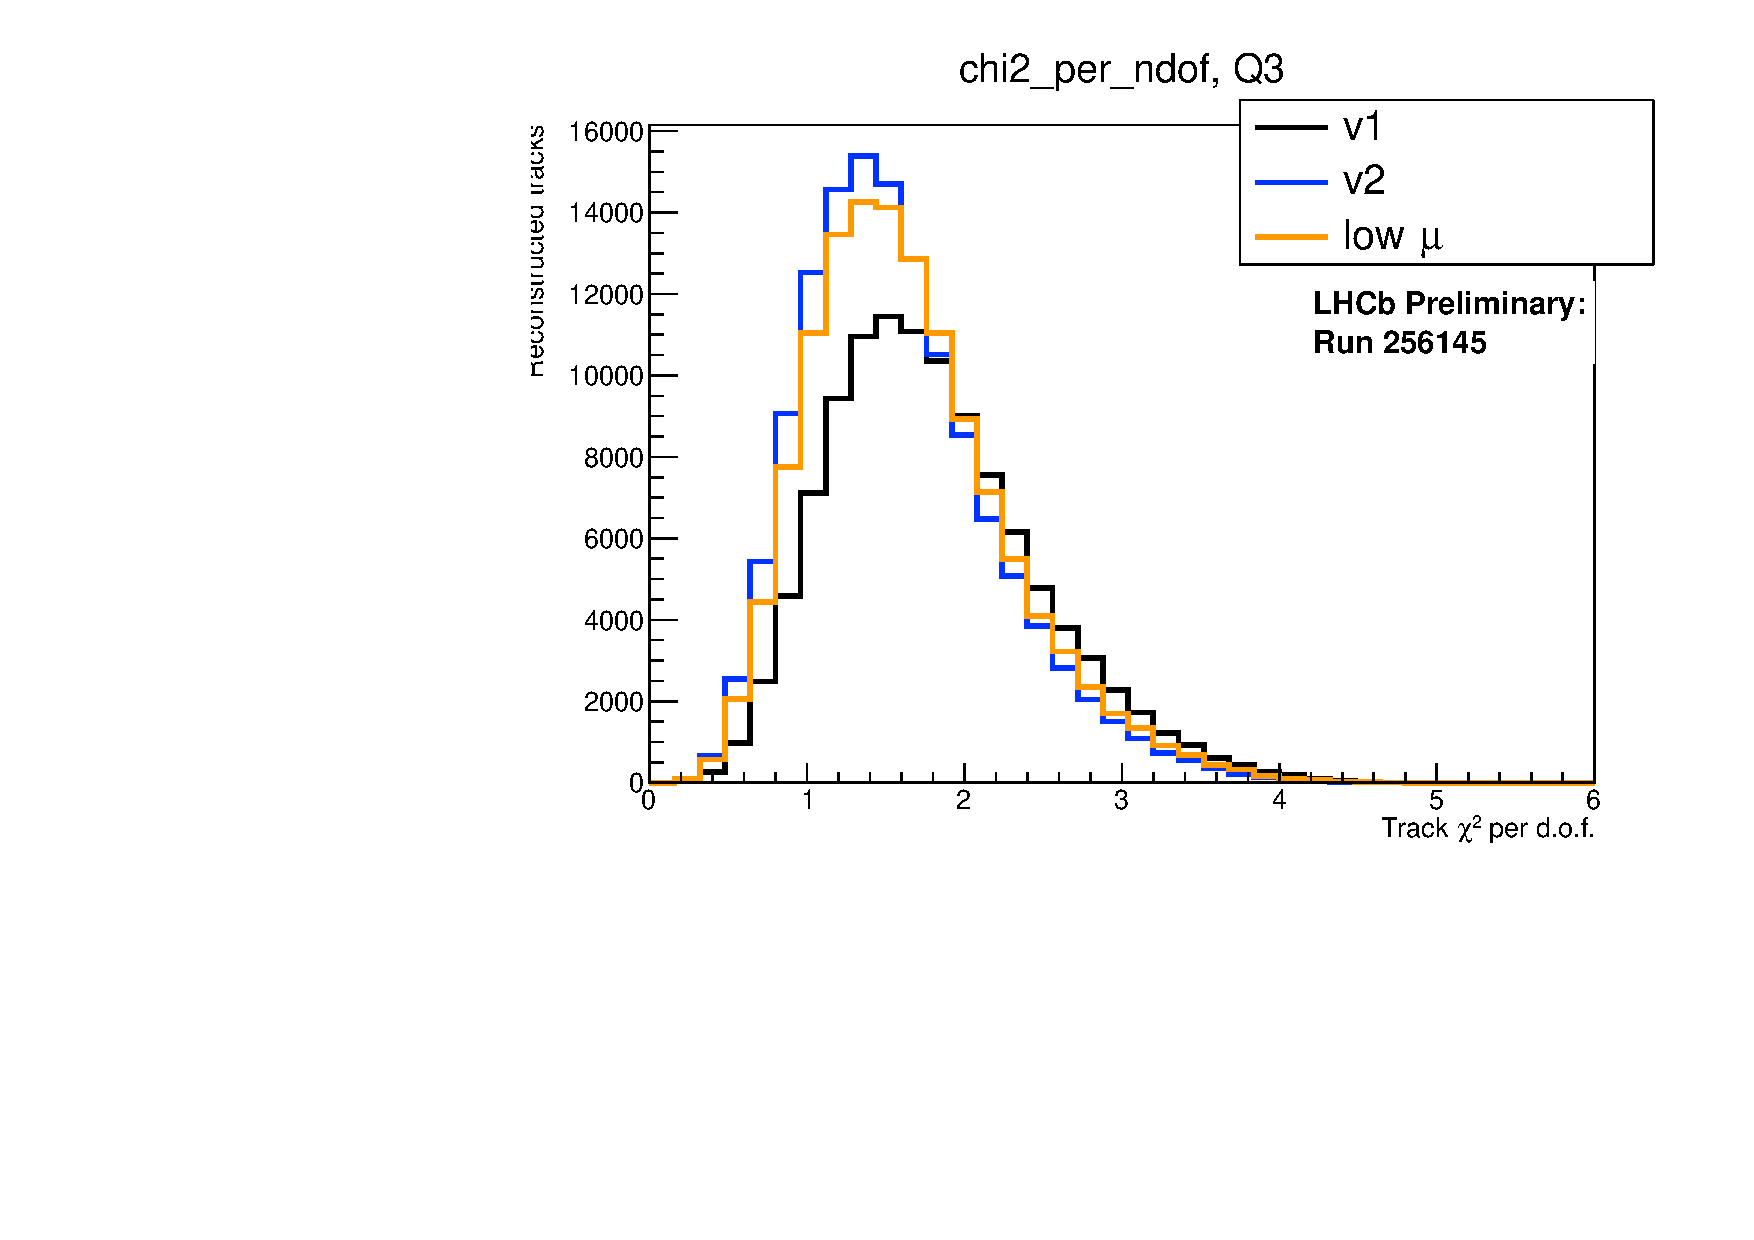
\includegraphics[width=0.9\textwidth]{2023-mar-9-DPG/chi2_per_ndof_Q3.pdf}
        \caption{track $\chi^2$ per dof comparing each alignment for Quarter 3.}
      \end{figure}
    \end{column}
    \begin{column}{0.48\textwidth}
      \begin{figure}
        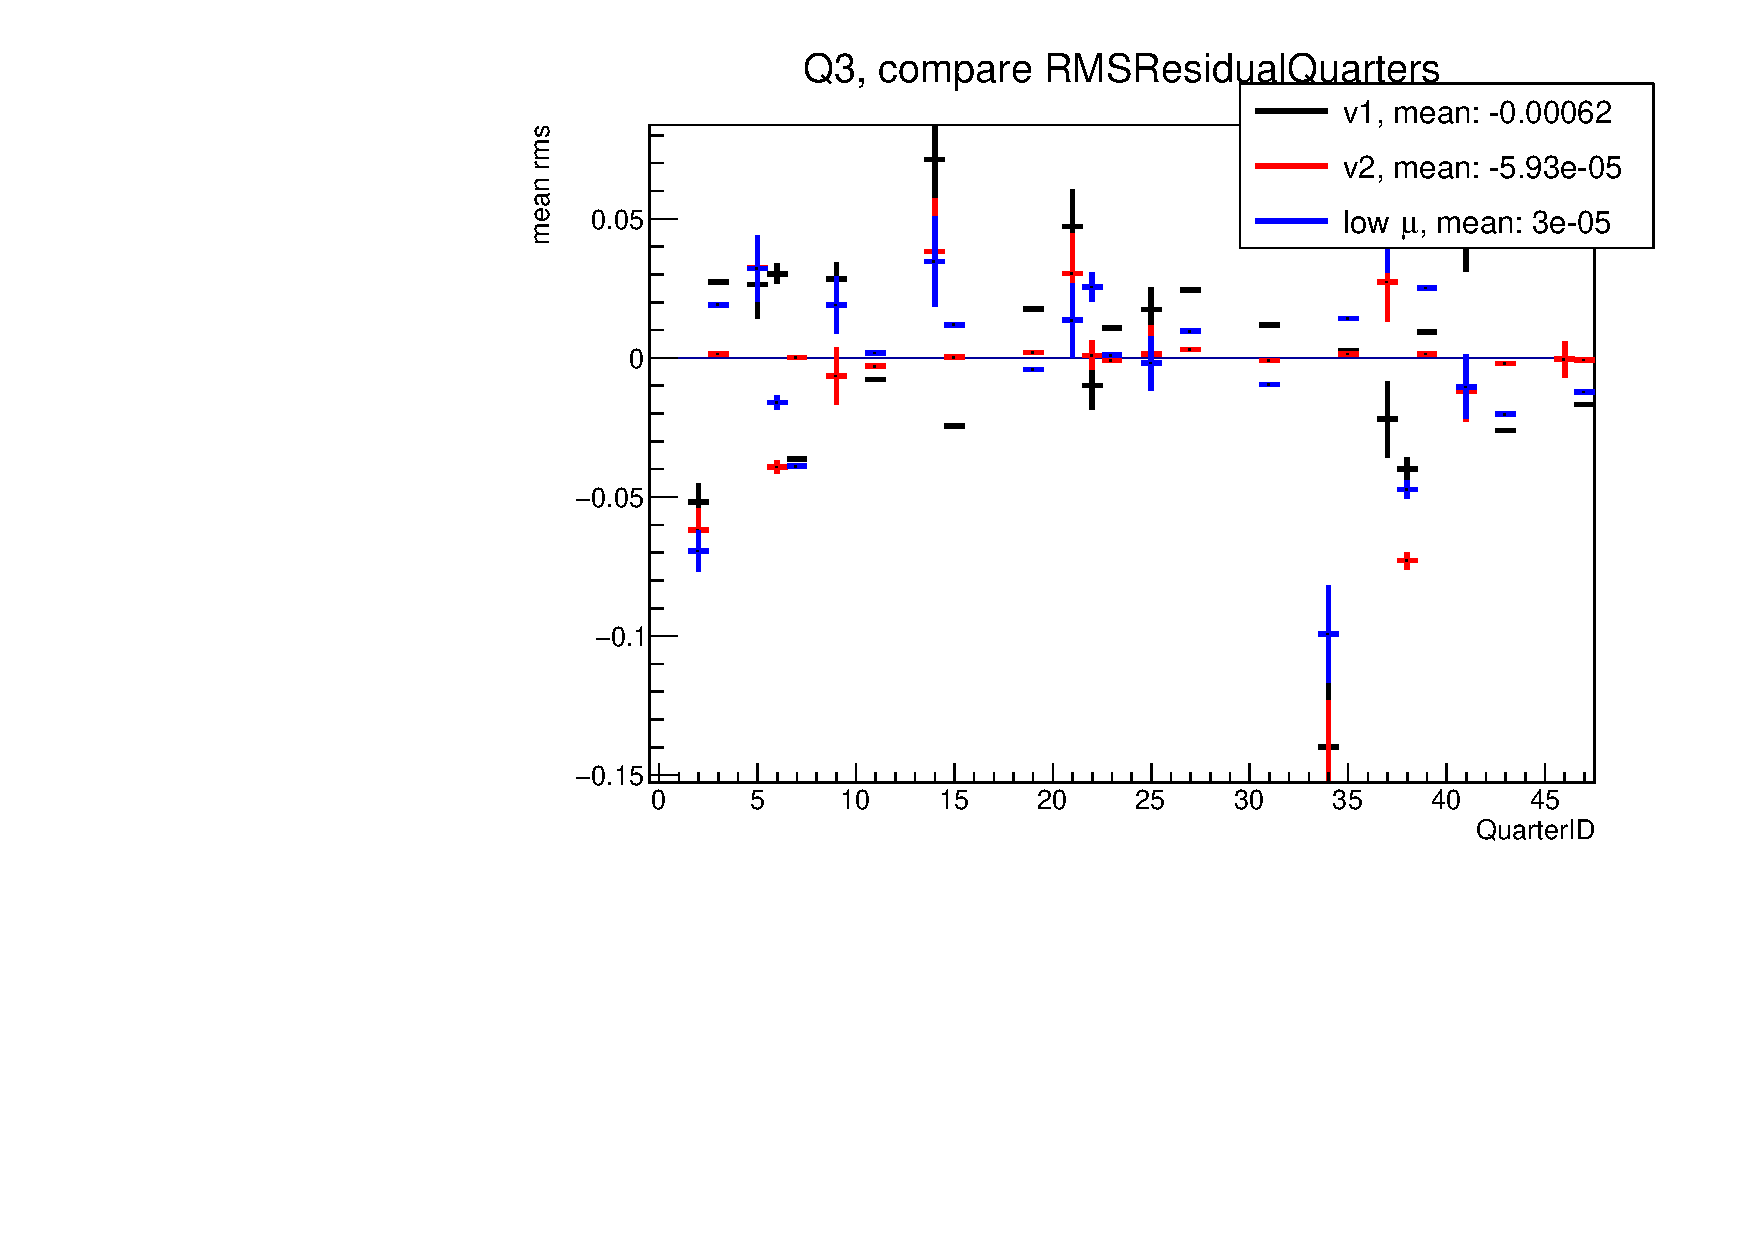
\includegraphics[width=0.9\textwidth]{2023-mar-9-DPG/RMSResidualQuarters_Q3.pdf}
        \caption{Residual in each module for each alignment in Quarter 3.}
      \end{figure}
    \end{column}
  \end{columns}
\end{frame}

% \begin{frame}\frametitle{}
%   \begin{columns}
%     \begin{column}[c]{0.48\textwidth}
%       \begin{figure}
%         \centering
%         \includegraphics[width=0.9\textwidth]{.pdf}
%         \caption{node X vs node Y vor v2 alignment.}
%       \end{figure}
%     \end{column}
%     \begin{column}{0.48\textwidth}
%       \begin{figure}
%         \includegraphics[width=0.9\textwidth]{.pdf}
%         \caption{node X vs node Y on Minbias, MagDown sample}
%       \end{figure}
%     \end{column}
%   \end{columns}
% \end{frame}
%
% \begin{frame}\frametitle{}
%   \begin{columns}
%     \begin{column}[c]{0.48\textwidth}
%       \begin{figure}
%         \centering
%         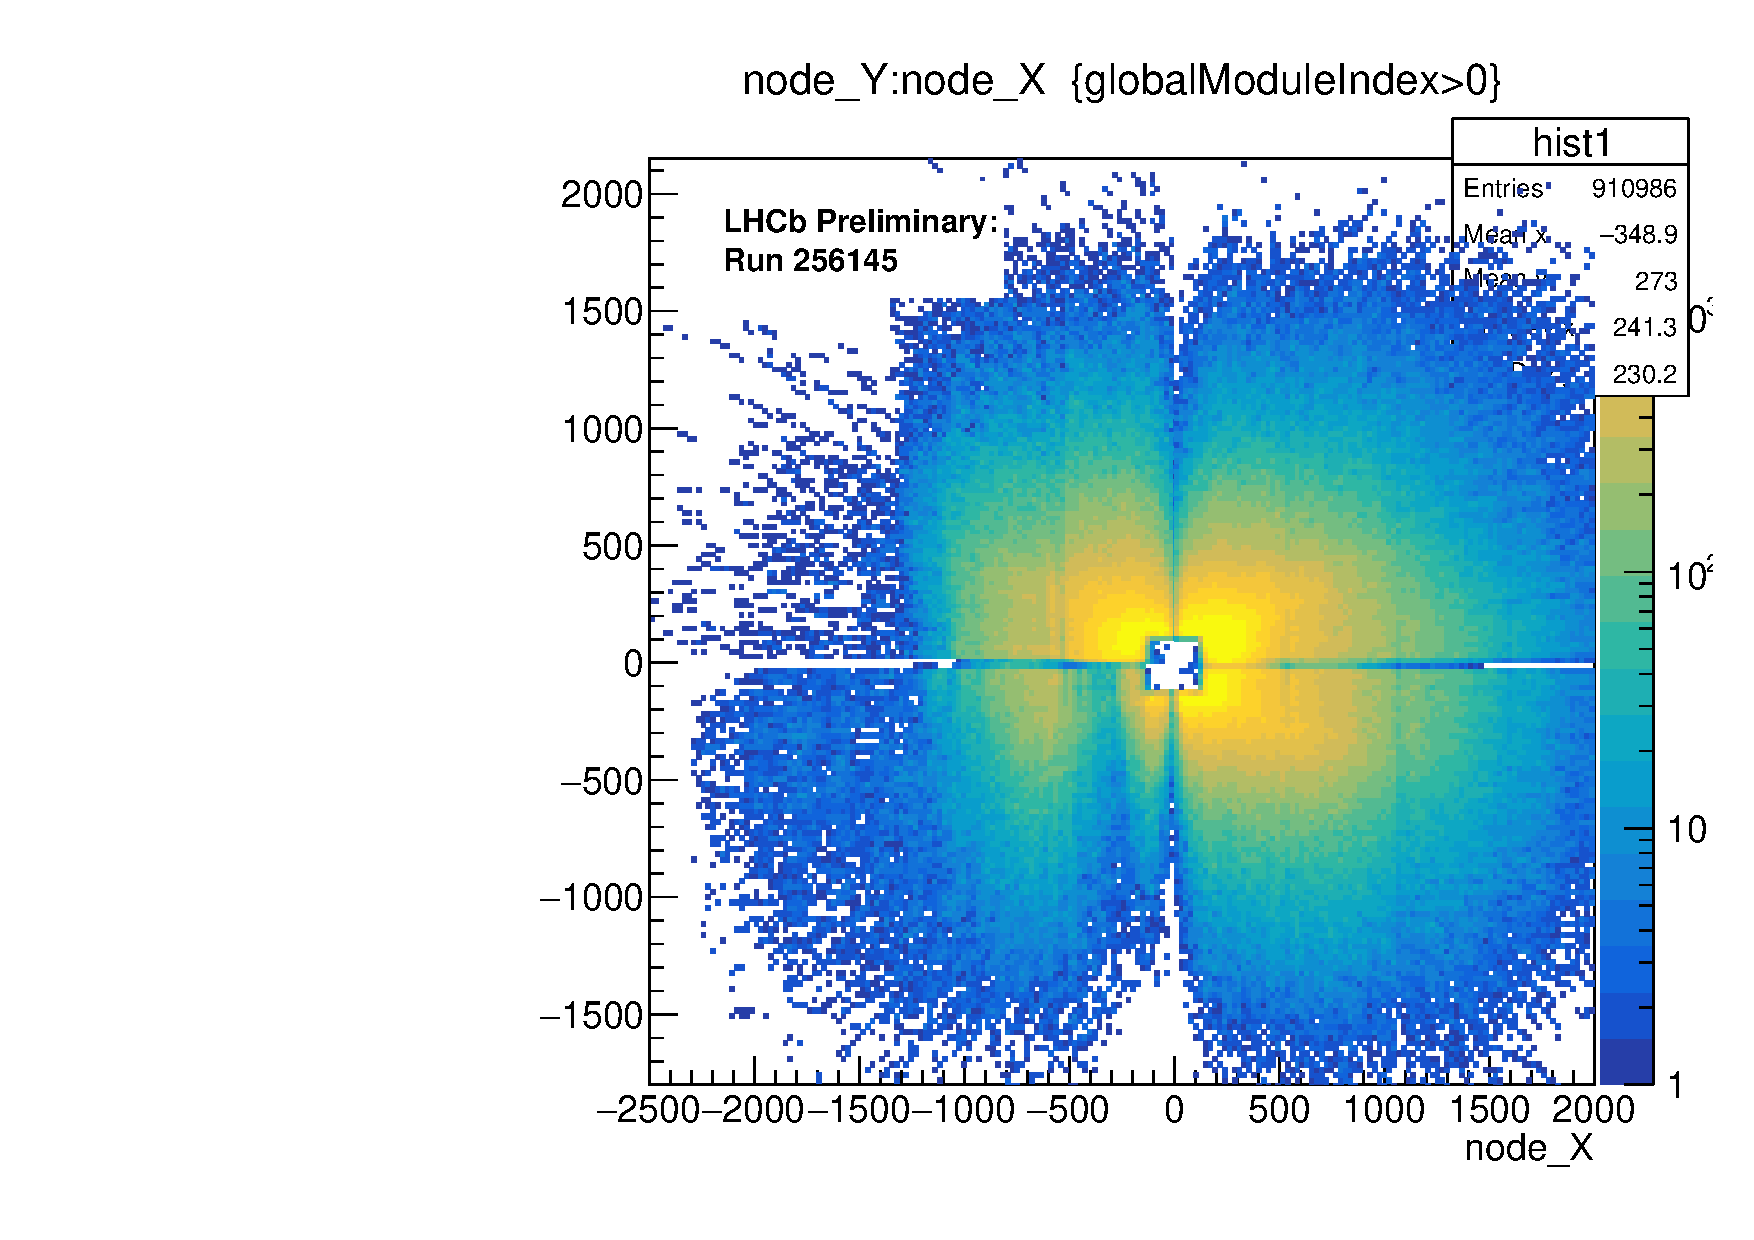
\includegraphics[width=0.9\textwidth]{2023-feb-07/combining_2D_nodeXY_v2.pdf}
%         \caption{node X vs node Y vor v2 alignment.}
%       \end{figure}
%     \end{column}
%     \begin{column}{0.48\textwidth}
%       \begin{figure}
%         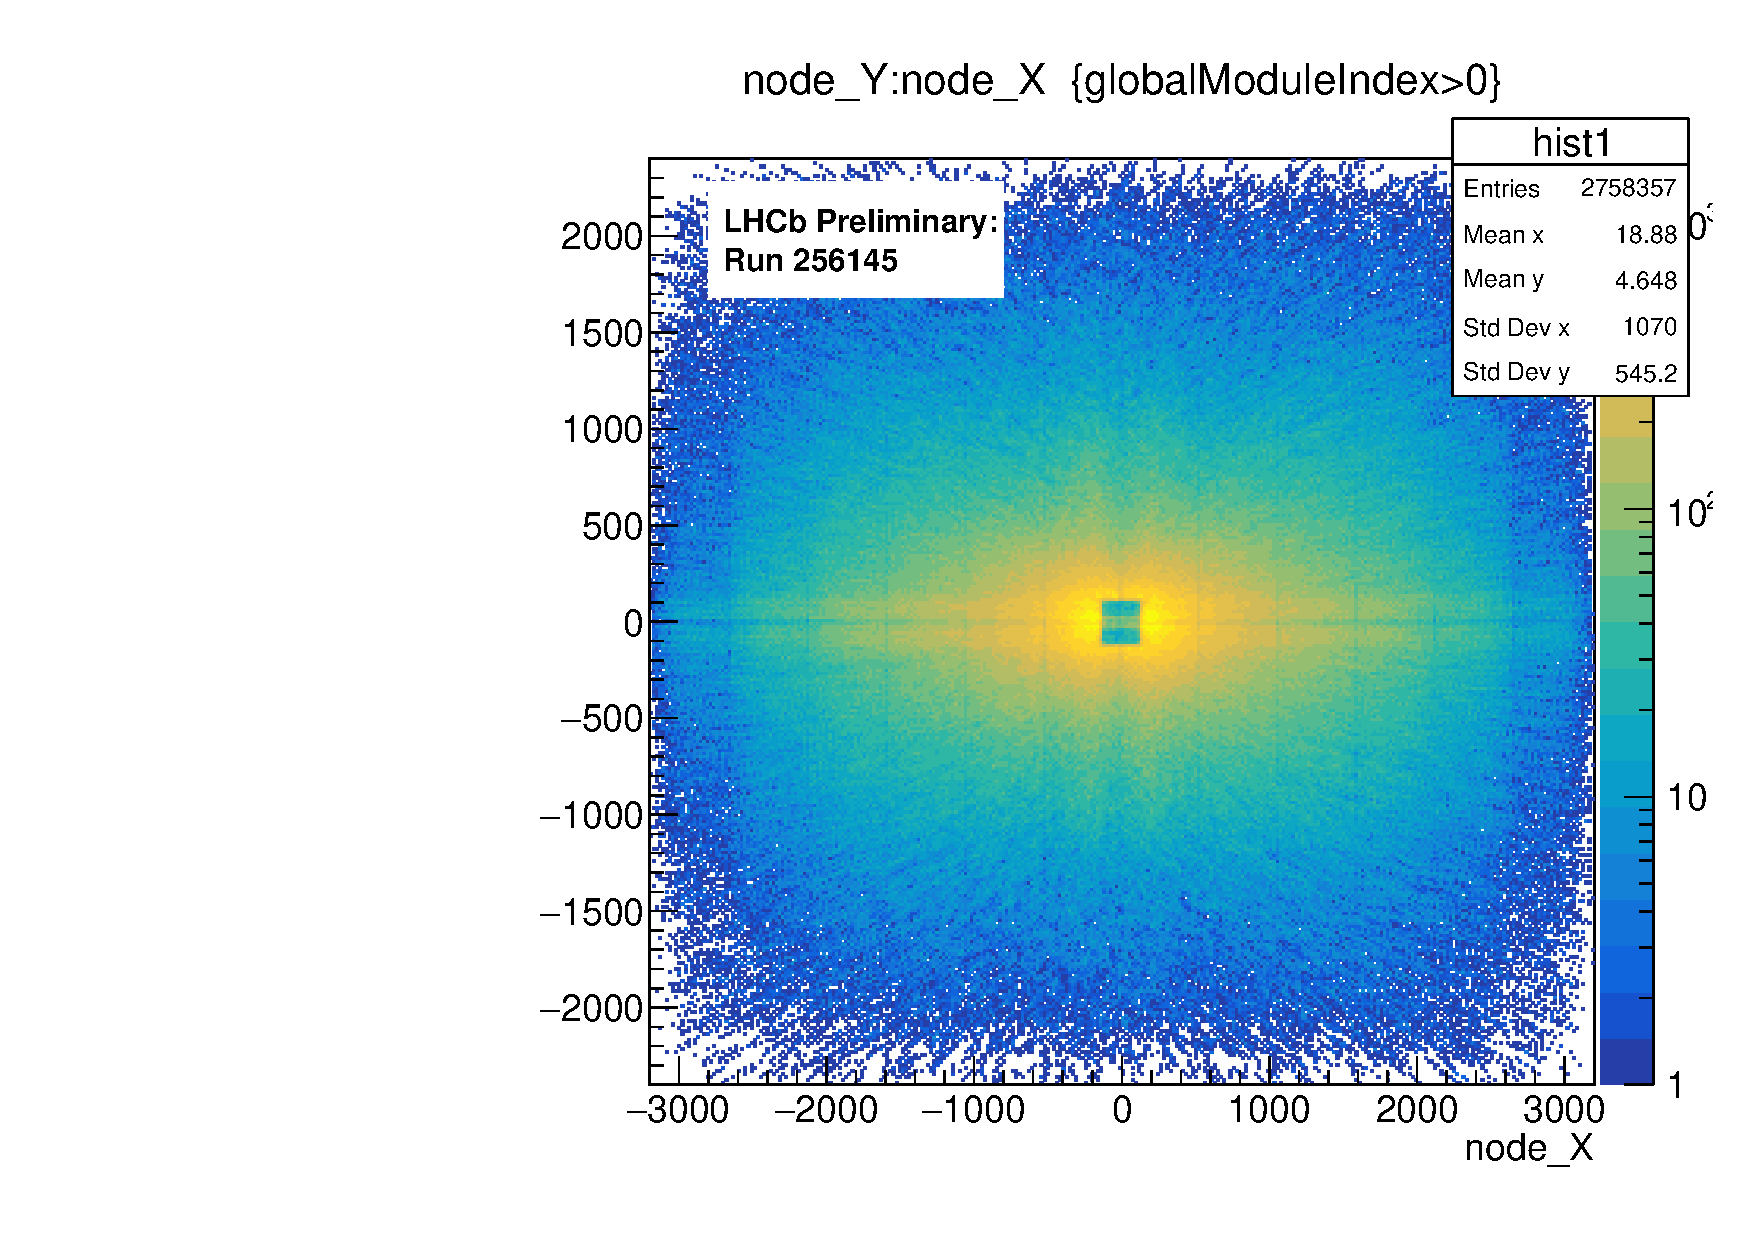
\includegraphics[width=0.9\textwidth]{2023-feb-07/nodeXY_MC.pdf}
%         \caption{node X vs node Y on Minbias, MagDown sample}
%       \end{figure}
%     \end{column}
%   \end{columns}
% \end{frame}



\begin{frame}\frametitle{Conclusion}
  \begin{itemize}
    \item $\bullet$\, text
  \end{itemize}
\end{frame}

\begin{frame}\frametitle{Sources}
  \begin{itemize}
    \item $\bullet$\,SciFi Conference Talk: \url{https://twiki.cern.ch/twiki/pub/LHCb/SciFiConference/fee_2018.pdf}
    \item $\bullet$\,LHCb SciFi: From performance requirements to an operational detector: \url{https://indico.cern.ch/event/1163878/}
  \end{itemize}
\end{frame}

\end{document}
